\section{LOG Natural Logarithm Function}

\subsection{Usage}

Computes the \verb|log| function for its argument.  The general
syntax for its use is
\begin{verbatim}
  y = log(x)
\end{verbatim}
where \verb|x| is an \verb|n|-dimensional array of numerical type.
Integer types are promoted to the \verb|double| type prior to
calculation of the \verb|log| function.  Output \verb|y| is of the
same size as the input \verb|x|. For strictly positive, real inputs, 
the output type is the same as the input.
For negative and complex arguments, the output is complex.
\subsection{Function Internals}

Mathematically, the \verb|log| function is defined for all real
valued arguments \verb|x| by the integral
\[
  \log x \equiv \int_1^{x} \frac{d\,t}{t}.
\]
For complex-valued arguments, \verb|z|, the complex logarithm is
defined as
\[
  \log z \equiv \log |z| + i \arg z,
\]
where \verb|arg| is the complex argument of \verb|z|.
\subsection{Example}

The following piece of code plots the real-valued \verb|log|
function over the interval \verb|[1,100]|:
@>


\centerline{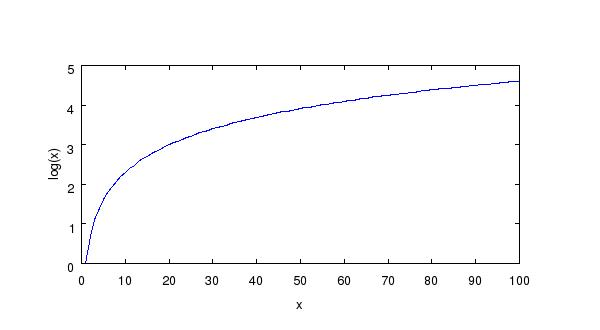
\includegraphics[width=8cm]{logplot}}

